% Created by tikzDevice version 0.7.0 on 2014-04-27 13:00:09
% !TEX encoding = UTF-8 Unicode
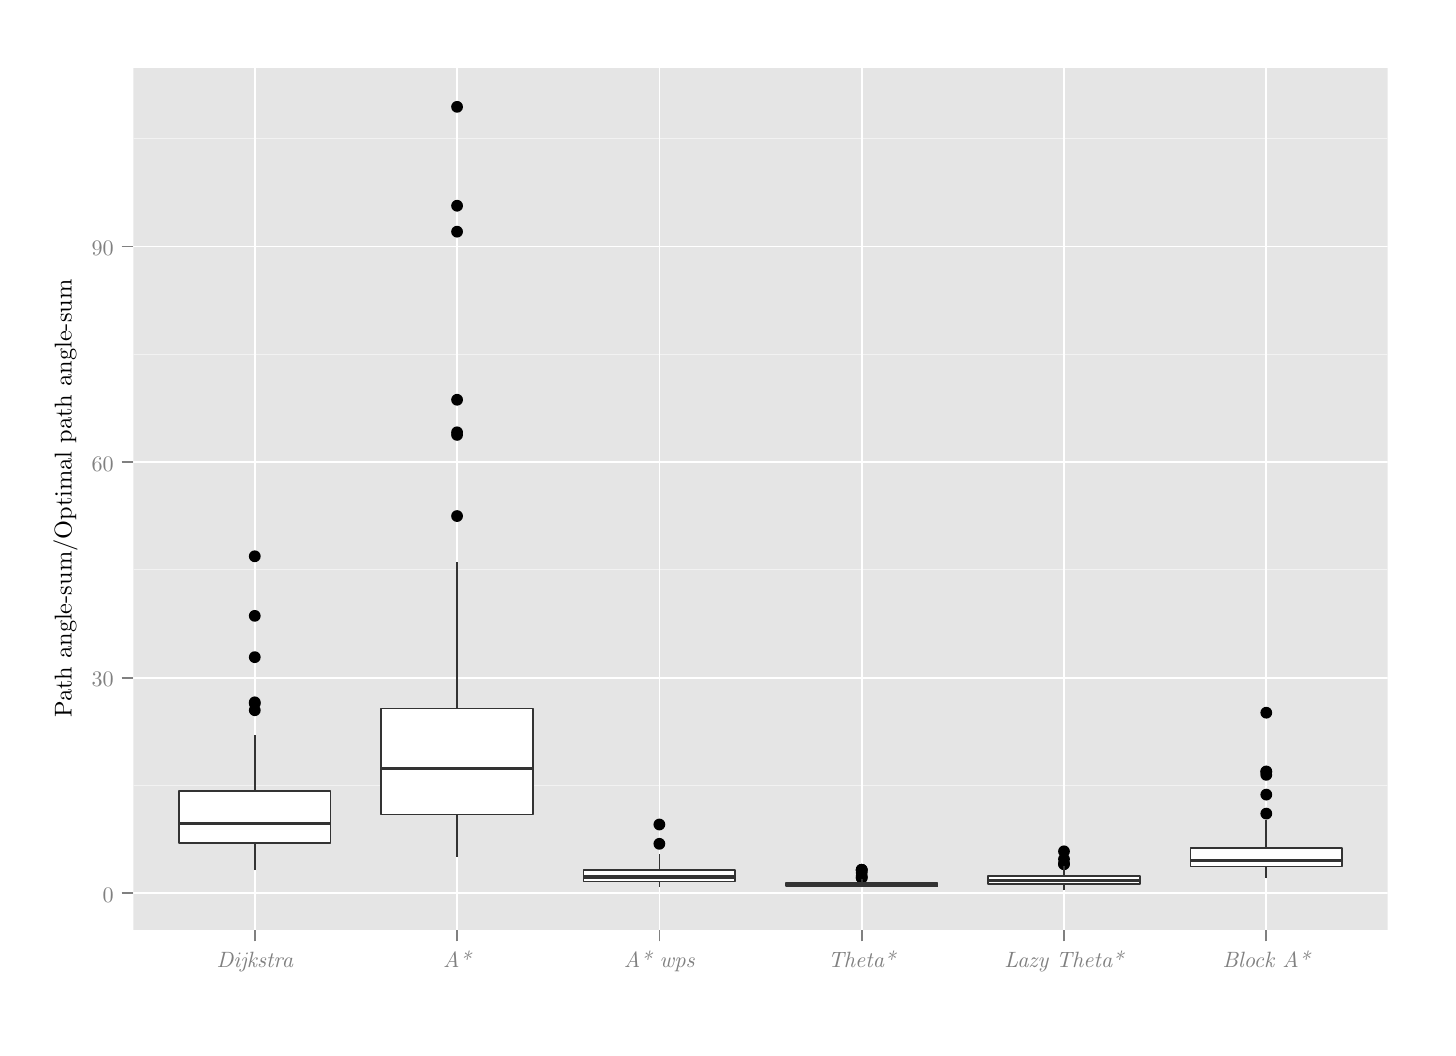
\begin{tikzpicture}[x=1pt,y=1pt]
\definecolor[named]{fillColor}{rgb}{1.00,1.00,1.00}
\path[use as bounding box,fill=fillColor,fill opacity=0.00] (0,0) rectangle (505.89,361.35);
\begin{scope}
\path[clip] (  0.00,  0.00) rectangle (505.89,361.35);
\definecolor[named]{drawColor}{rgb}{1.00,1.00,1.00}
\definecolor[named]{fillColor}{rgb}{1.00,1.00,1.00}

\path[draw=drawColor,line width= 0.6pt,line join=round,line cap=round,fill=fillColor] (  0.00, -0.00) rectangle (505.89,361.35);
\end{scope}
\begin{scope}
\path[clip] ( 38.20, 35.41) rectangle (491.44,346.90);
\definecolor[named]{fillColor}{rgb}{0.90,0.90,0.90}

\path[fill=fillColor] ( 38.20, 35.41) rectangle (491.44,346.90);
\definecolor[named]{drawColor}{rgb}{0.95,0.95,0.95}

\path[draw=drawColor,line width= 0.3pt,line join=round] ( 38.20, 87.50) --
	(491.44, 87.50);

\path[draw=drawColor,line width= 0.3pt,line join=round] ( 38.20,165.42) --
	(491.44,165.42);

\path[draw=drawColor,line width= 0.3pt,line join=round] ( 38.20,243.33) --
	(491.44,243.33);

\path[draw=drawColor,line width= 0.3pt,line join=round] ( 38.20,321.24) --
	(491.44,321.24);
\definecolor[named]{drawColor}{rgb}{1.00,1.00,1.00}

\path[draw=drawColor,line width= 0.6pt,line join=round] ( 38.20, 48.55) --
	(491.44, 48.55);

\path[draw=drawColor,line width= 0.6pt,line join=round] ( 38.20,126.46) --
	(491.44,126.46);

\path[draw=drawColor,line width= 0.6pt,line join=round] ( 38.20,204.37) --
	(491.44,204.37);

\path[draw=drawColor,line width= 0.6pt,line join=round] ( 38.20,282.29) --
	(491.44,282.29);

\path[draw=drawColor,line width= 0.6pt,line join=round] ( 82.06, 35.41) --
	( 82.06,346.90);

\path[draw=drawColor,line width= 0.6pt,line join=round] (155.16, 35.41) --
	(155.16,346.90);

\path[draw=drawColor,line width= 0.6pt,line join=round] (228.26, 35.41) --
	(228.26,346.90);

\path[draw=drawColor,line width= 0.6pt,line join=round] (301.37, 35.41) --
	(301.37,346.90);

\path[draw=drawColor,line width= 0.6pt,line join=round] (374.47, 35.41) --
	(374.47,346.90);

\path[draw=drawColor,line width= 0.6pt,line join=round] (447.57, 35.41) --
	(447.57,346.90);
\definecolor[named]{fillColor}{rgb}{0.00,0.00,0.00}

\path[fill=fillColor] ( 82.06,117.14) circle (  2.13);

\path[fill=fillColor] ( 82.06,170.34) circle (  2.13);

\path[fill=fillColor] ( 82.06,133.88) circle (  2.13);

\path[fill=fillColor] ( 82.06,148.81) circle (  2.13);

\path[fill=fillColor] ( 82.06,114.71) circle (  2.13);

\path[fill=fillColor] ( 82.06,117.56) circle (  2.13);
\definecolor[named]{drawColor}{rgb}{0.20,0.20,0.20}
\definecolor[named]{fillColor}{rgb}{0.20,0.20,0.20}

\path[draw=drawColor,line width= 0.6pt,line join=round,fill=fillColor] ( 82.06, 85.52) -- ( 82.06,105.74);

\path[draw=drawColor,line width= 0.6pt,line join=round,fill=fillColor] ( 82.06, 66.76) -- ( 82.06, 56.91);
\definecolor[named]{fillColor}{rgb}{1.00,1.00,1.00}

\path[draw=drawColor,line width= 0.6pt,line join=round,line cap=round,fill=fillColor] ( 54.64, 85.52) --
	( 54.64, 66.76) --
	(109.47, 66.76) --
	(109.47, 85.52) --
	( 54.64, 85.52) --
	cycle;
\definecolor[named]{fillColor}{rgb}{0.20,0.20,0.20}

\path[draw=drawColor,line width= 1.1pt,line join=round,fill=fillColor] ( 54.64, 73.64) -- (109.47, 73.64);
\definecolor[named]{fillColor}{rgb}{0.00,0.00,0.00}

\path[fill=fillColor] (155.16,215.13) circle (  2.13);

\path[fill=fillColor] (155.16,226.89) circle (  2.13);

\path[fill=fillColor] (155.16,332.74) circle (  2.13);

\path[fill=fillColor] (155.16,184.87) circle (  2.13);

\path[fill=fillColor] (155.16,214.19) circle (  2.13);

\path[fill=fillColor] (155.16,287.63) circle (  2.13);

\path[fill=fillColor] (155.16,297.00) circle (  2.13);
\definecolor[named]{fillColor}{rgb}{0.20,0.20,0.20}

\path[draw=drawColor,line width= 0.6pt,line join=round,fill=fillColor] (155.16,115.29) -- (155.16,168.14);

\path[draw=drawColor,line width= 0.6pt,line join=round,fill=fillColor] (155.16, 77.00) -- (155.16, 61.71);
\definecolor[named]{fillColor}{rgb}{1.00,1.00,1.00}

\path[draw=drawColor,line width= 0.6pt,line join=round,line cap=round,fill=fillColor] (127.75,115.29) --
	(127.75, 77.00) --
	(182.58, 77.00) --
	(182.58,115.29) --
	(127.75,115.29) --
	cycle;
\definecolor[named]{fillColor}{rgb}{0.20,0.20,0.20}

\path[draw=drawColor,line width= 1.1pt,line join=round,fill=fillColor] (127.75, 93.53) -- (182.58, 93.53);
\definecolor[named]{fillColor}{rgb}{0.00,0.00,0.00}

\path[fill=fillColor] (228.26, 66.44) circle (  2.13);

\path[fill=fillColor] (228.26, 73.42) circle (  2.13);
\definecolor[named]{fillColor}{rgb}{0.20,0.20,0.20}

\path[draw=drawColor,line width= 0.6pt,line join=round,fill=fillColor] (228.26, 57.01) -- (228.26, 62.74);

\path[draw=drawColor,line width= 0.6pt,line join=round,fill=fillColor] (228.26, 52.84) -- (228.26, 50.88);
\definecolor[named]{fillColor}{rgb}{1.00,1.00,1.00}

\path[draw=drawColor,line width= 0.6pt,line join=round,line cap=round,fill=fillColor] (200.85, 57.01) --
	(200.85, 52.84) --
	(255.68, 52.84) --
	(255.68, 57.01) --
	(200.85, 57.01) --
	cycle;
\definecolor[named]{fillColor}{rgb}{0.20,0.20,0.20}

\path[draw=drawColor,line width= 1.1pt,line join=round,fill=fillColor] (200.85, 54.44) -- (255.68, 54.44);
\definecolor[named]{fillColor}{rgb}{0.00,0.00,0.00}

\path[fill=fillColor] (301.37, 54.13) circle (  2.13);

\path[fill=fillColor] (301.37, 57.05) circle (  2.13);

\path[fill=fillColor] (301.37, 56.01) circle (  2.13);

\path[fill=fillColor] (301.37, 54.18) circle (  2.13);

\path[fill=fillColor] (301.37, 57.02) circle (  2.13);

\path[fill=fillColor] (301.37, 54.78) circle (  2.13);

\path[fill=fillColor] (301.37, 57.04) circle (  2.13);
\definecolor[named]{fillColor}{rgb}{0.20,0.20,0.20}

\path[draw=drawColor,line width= 0.6pt,line join=round,fill=fillColor] (301.37, 52.34) -- (301.37, 53.86);

\path[draw=drawColor,line width= 0.6pt,line join=round,fill=fillColor] (301.37, 51.18) -- (301.37, 50.67);
\definecolor[named]{fillColor}{rgb}{1.00,1.00,1.00}

\path[draw=drawColor,line width= 0.6pt,line join=round,line cap=round,fill=fillColor] (273.95, 52.34) --
	(273.95, 51.18) --
	(328.78, 51.18) --
	(328.78, 52.34) --
	(273.95, 52.34) --
	cycle;
\definecolor[named]{fillColor}{rgb}{0.20,0.20,0.20}

\path[draw=drawColor,line width= 1.1pt,line join=round,fill=fillColor] (273.95, 51.47) -- (328.78, 51.47);
\definecolor[named]{fillColor}{rgb}{0.00,0.00,0.00}

\path[fill=fillColor] (374.47, 63.72) circle (  2.13);

\path[fill=fillColor] (374.47, 59.29) circle (  2.13);

\path[fill=fillColor] (374.47, 59.04) circle (  2.13);

\path[fill=fillColor] (374.47, 60.91) circle (  2.13);
\definecolor[named]{fillColor}{rgb}{0.20,0.20,0.20}

\path[draw=drawColor,line width= 0.6pt,line join=round,fill=fillColor] (374.47, 54.72) -- (374.47, 58.39);

\path[draw=drawColor,line width= 0.6pt,line join=round,fill=fillColor] (374.47, 51.85) -- (374.47, 49.57);
\definecolor[named]{fillColor}{rgb}{1.00,1.00,1.00}

\path[draw=drawColor,line width= 0.6pt,line join=round,line cap=round,fill=fillColor] (347.06, 54.72) --
	(347.06, 51.85) --
	(401.88, 51.85) --
	(401.88, 54.72) --
	(347.06, 54.72) --
	cycle;
\definecolor[named]{fillColor}{rgb}{0.20,0.20,0.20}

\path[draw=drawColor,line width= 1.1pt,line join=round,fill=fillColor] (347.06, 53.08) -- (401.88, 53.08);
\definecolor[named]{fillColor}{rgb}{0.00,0.00,0.00}

\path[fill=fillColor] (447.57, 77.35) circle (  2.13);

\path[fill=fillColor] (447.57,113.81) circle (  2.13);

\path[fill=fillColor] (447.57, 84.21) circle (  2.13);

\path[fill=fillColor] (447.57, 92.46) circle (  2.13);

\path[fill=fillColor] (447.57, 91.36) circle (  2.13);

\path[fill=fillColor] (447.57, 92.58) circle (  2.13);
\definecolor[named]{fillColor}{rgb}{0.20,0.20,0.20}

\path[draw=drawColor,line width= 0.6pt,line join=round,fill=fillColor] (447.57, 65.04) -- (447.57, 75.15);

\path[draw=drawColor,line width= 0.6pt,line join=round,fill=fillColor] (447.57, 58.28) -- (447.57, 53.99);
\definecolor[named]{fillColor}{rgb}{1.00,1.00,1.00}

\path[draw=drawColor,line width= 0.6pt,line join=round,line cap=round,fill=fillColor] (420.16, 65.04) --
	(420.16, 58.28) --
	(474.99, 58.28) --
	(474.99, 65.04) --
	(420.16, 65.04) --
	cycle;
\definecolor[named]{fillColor}{rgb}{0.20,0.20,0.20}

\path[draw=drawColor,line width= 1.1pt,line join=round,fill=fillColor] (420.16, 60.45) -- (474.99, 60.45);
\end{scope}
\begin{scope}
\path[clip] (  0.00,  0.00) rectangle (505.89,361.35);
\definecolor[named]{drawColor}{rgb}{0.50,0.50,0.50}

\node[text=drawColor,anchor=base east,inner sep=0pt, outer sep=0pt, scale=  0.80] at ( 31.08, 45.24) {0};

\node[text=drawColor,anchor=base east,inner sep=0pt, outer sep=0pt, scale=  0.80] at ( 31.08,123.15) {30};

\node[text=drawColor,anchor=base east,inner sep=0pt, outer sep=0pt, scale=  0.80] at ( 31.08,201.07) {60};

\node[text=drawColor,anchor=base east,inner sep=0pt, outer sep=0pt, scale=  0.80] at ( 31.08,278.98) {90};
\end{scope}
\begin{scope}
\path[clip] (  0.00,  0.00) rectangle (505.89,361.35);
\definecolor[named]{drawColor}{rgb}{0.50,0.50,0.50}

\path[draw=drawColor,line width= 0.6pt,line join=round] ( 33.93, 48.55) --
	( 38.20, 48.55);

\path[draw=drawColor,line width= 0.6pt,line join=round] ( 33.93,126.46) --
	( 38.20,126.46);

\path[draw=drawColor,line width= 0.6pt,line join=round] ( 33.93,204.37) --
	( 38.20,204.37);

\path[draw=drawColor,line width= 0.6pt,line join=round] ( 33.93,282.29) --
	( 38.20,282.29);
\end{scope}
\begin{scope}
\path[clip] (  0.00,  0.00) rectangle (505.89,361.35);
\definecolor[named]{drawColor}{rgb}{0.50,0.50,0.50}

\path[draw=drawColor,line width= 0.6pt,line join=round] ( 82.06, 31.14) --
	( 82.06, 35.41);

\path[draw=drawColor,line width= 0.6pt,line join=round] (155.16, 31.14) --
	(155.16, 35.41);

\path[draw=drawColor,line width= 0.6pt,line join=round] (228.26, 31.14) --
	(228.26, 35.41);

\path[draw=drawColor,line width= 0.6pt,line join=round] (301.37, 31.14) --
	(301.37, 35.41);

\path[draw=drawColor,line width= 0.6pt,line join=round] (374.47, 31.14) --
	(374.47, 35.41);

\path[draw=drawColor,line width= 0.6pt,line join=round] (447.57, 31.14) --
	(447.57, 35.41);
\end{scope}
\begin{scope}
\path[clip] (  0.00,  0.00) rectangle (505.89,361.35);
\definecolor[named]{drawColor}{rgb}{0.50,0.50,0.50}

\node[text=drawColor,anchor=base,inner sep=0pt, outer sep=0pt, scale=  0.80] at ( 82.06, 21.69) {{\em Dijkstra}};

\node[text=drawColor,anchor=base,inner sep=0pt, outer sep=0pt, scale=  0.80] at (155.16, 21.69) {{\em A*}};

\node[text=drawColor,anchor=base,inner sep=0pt, outer sep=0pt, scale=  0.80] at (228.26, 21.69) {{\em A* wps}};

\node[text=drawColor,anchor=base,inner sep=0pt, outer sep=0pt, scale=  0.80] at (301.37, 21.69) {{\em Theta*}};

\node[text=drawColor,anchor=base,inner sep=0pt, outer sep=0pt, scale=  0.80] at (374.47, 21.69) {{\em Lazy Theta*}};

\node[text=drawColor,anchor=base,inner sep=0pt, outer sep=0pt, scale=  0.80] at (447.57, 21.69) {{\em Block A*}};
\end{scope}
\begin{scope}
\path[clip] (  0.00,  0.00) rectangle (505.89,361.35);
\definecolor[named]{drawColor}{rgb}{0.00,0.00,0.00}

\node[text=drawColor,rotate= 90.00,anchor=base,inner sep=0pt, outer sep=0pt, scale=  0.88] at ( 15.90,191.15) {Path angle-sum/Optimal path angle-sum};
\end{scope}
\end{tikzpicture}
